\documentclass{article}
\usepackage{tikz}

\begin{document}

\begin{figure}[h]
    \centering
    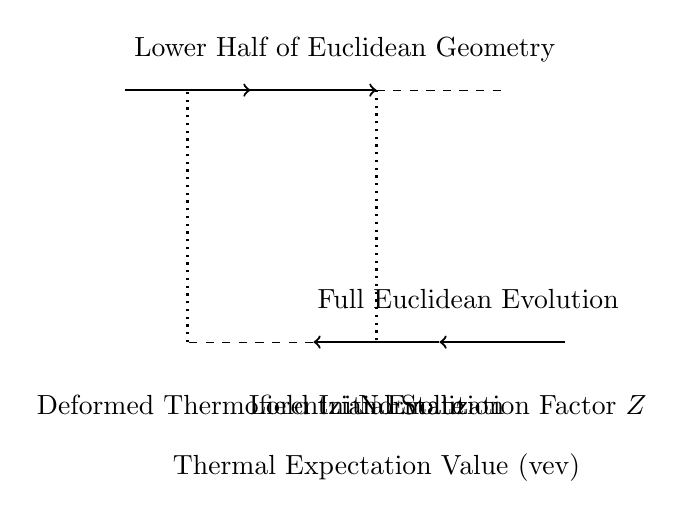
\begin{tikzpicture}[scale=0.8]

        % Left side: Lower half of Euclidean geometry with Lorentzian evolution
        \node[anchor=north west] at (0,2) {Lower Half of Euclidean Geometry};
        \draw[thick,->] (0,1) -- (2,1);
        \draw[thick,->] (2,1) -- (4,1);
        \draw[dashed] (4,1) -- (6,1);

        % Right side: Full Euclidean evolution
        \node[anchor=north east] at (8,-2) {Full Euclidean Evolution};
        \draw[thick,->] (7,-3) -- (5,-3);
        \draw[thick,->] (5,-3) -- (3,-3);
        \draw[dashed] (3,-3) -- (1,-3);

        % Connecting lines
        \draw[thick,dotted] (4,1) -- (4,-3);
        \draw[thick,dotted] (1,-3) -- (1,1);

        % Labels
        \node at (4,-4) {Lorentzian Evolution};
        \node at (2,-4) {Deformed Thermofield Initial State};
        \node at (6,-4) {Normalization Factor \( Z \)};
        \node at (4,-5) {Thermal Expectation Value (vev)};

    \end{tikzpicture}
    \caption{Comparison between Lower Half of Euclidean Geometry and Full Euclidean Evolution}
    \label{fig:euc_vs_lorentz}
\end{figure}

\end{document}